\begin{frame}{Fixing overconfidence in Dynamic Neural Networks}
    \textit{IEEE/CVF Winter Conference on Applications of Computer Vision (WACV) 2024
    }

    \begin{itemize}
        \item To decrease computational cost, we do not want to run network for more layers that required for the specific task
        \item To be able to know where to stop, the model needs good uncertainty estimates
        \item The paper aims to improve uncertainty estimates for a model
    \end{itemize}
    \begin{figure}
        \centering
        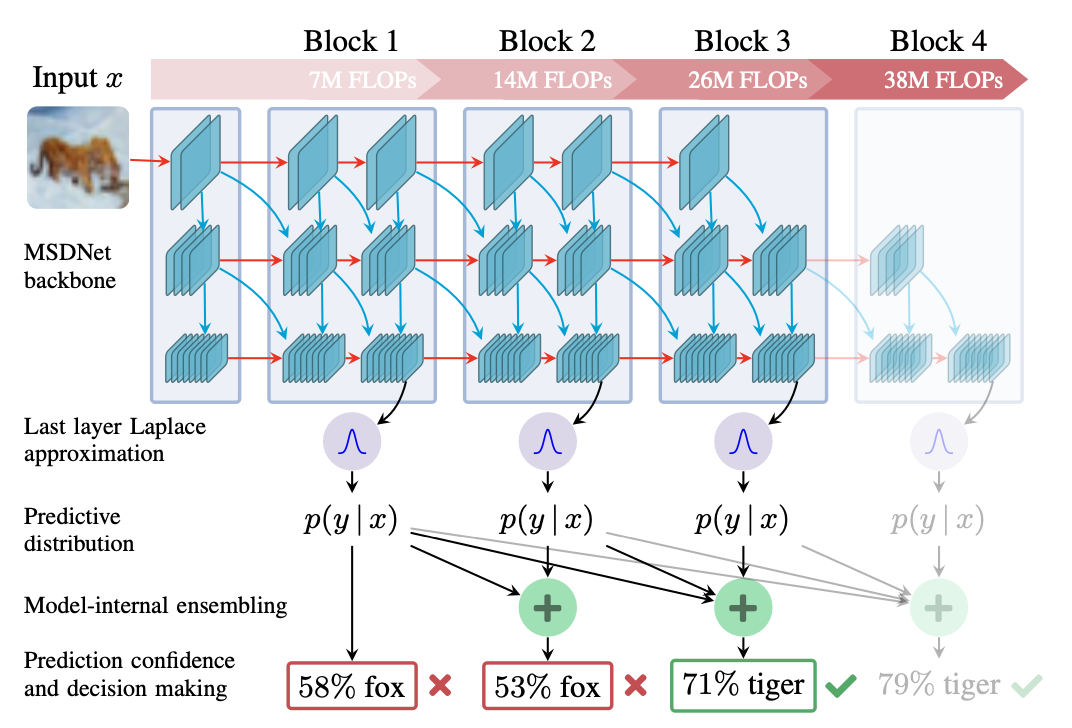
\includegraphics[width=0.4\linewidth]{Screenshot 2025-04-08 at 15.02.28.png}
        \caption{Increasing depth of dynamic neural network}
        \label{fig:enter-label}
    \end{figure}
\end{frame}

\begin{frame}{Background}

    \begin{itemize}
        \item Investigates image classification under budget restrictions \\
              \(\mathcal{D}_{\text{train}} = \left\{ (\mathbf{x}_i, \mathbf{y}_i) \right\}_{i=1}^{n_{\text{train}}}\)
        \item Budget B (FLOPs) must be distributed across a batch for highest possible accuracy
        \item With $n_{block}$ intermediate classifiers, the predictive distribution: \\
              \( p_k(\hat{\mathbf{y}}_i \mid \mathbf{x}_i),\; k = 1, 2, \ldots, n_{\text{block}} \)
        \item Feature representation on the last linear layer \\
              \( \phi_{i,k} = f_k(\mathbf{x}_i) \) with parameters \( \theta_k = \{ \mathbf{W}_k, \mathbf{b}_k \} \)
        \item Prediction of layer k: \\
              \( p_k(\hat{\mathbf{y}}_i \mid \mathbf{x}_i) = \text{softmax}(\hat{\mathbf{z}}_{i,k}), \text{ where } \hat{\mathbf{z}}_{i,k} = \mathbf{W}_k \boldsymbol{\phi}_{i,k} + \mathbf{b}_k \)



    \end{itemize}

\end{frame}

\begin{frame}{Aleatoric and epistemic uncertainty}
    \begin{itemize}
        \item Aleatoric uncertainty is related to randomness intrinsic to the task at hand and cannot be reduced.
        \item Epistemic uncertainty is related to our knowledge of the task and can be reduced by learning more about the task → more data
    \end{itemize}
    \begin{figure}
        \centering
        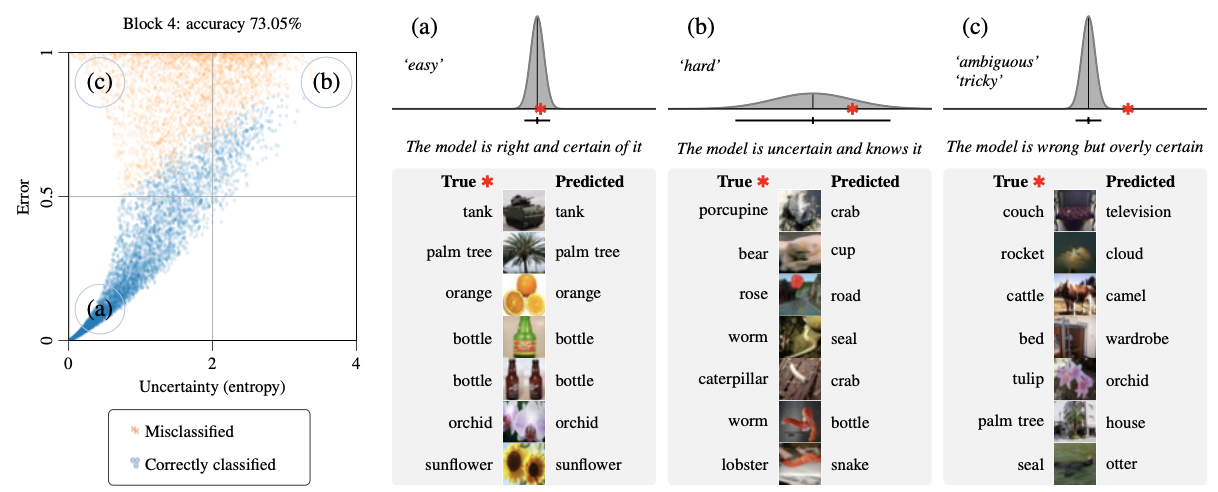
\includegraphics[width=0.7\linewidth]{Screenshot 2025-04-08 at 15.14.46.png}
        \label{fig:enter-label}
    \end{figure}

\end{frame}

\begin{frame}{Bayesian treatment of parameters}
    \[
        p(\boldsymbol{\theta} \mid \mathcal{D}_{\text{train}})
        = \frac{p(\mathcal{D}_{\text{train}} \mid \boldsymbol{\theta}) \, p(\boldsymbol{\theta})}{\int_{\boldsymbol{\theta}} p(\mathcal{D}_{\text{train}}, \boldsymbol{\theta}) \, d\boldsymbol{\theta}}
        = \frac{\text{[likelihood]} \times \text{[prior]}}{\text{[model evidence]}}
    \]


    \begin{itemize}
        \item Posterior distribution over the model parameters is intractable in deep learning
        \item Laplace approximation (second order Taylor expansion)
        \item MAP estimate can be found by maximising the unnormalised posterior:

              \[
                  \hat{\boldsymbol{\theta}} = \arg\max_{\boldsymbol{\theta}} \log p(\mathcal{D}_{\text{train}} \mid \boldsymbol{\theta}) + \log p(\boldsymbol{\theta})
              \]

              \[
                  p(\boldsymbol{\theta} \mid \mathcal{D}_{\text{train}}) \approx \mathcal{N}(\hat{\boldsymbol{\theta}}, \mathbf{H}^{-1})
              \]
    \end{itemize}
    \begin{figure}
        \centering
        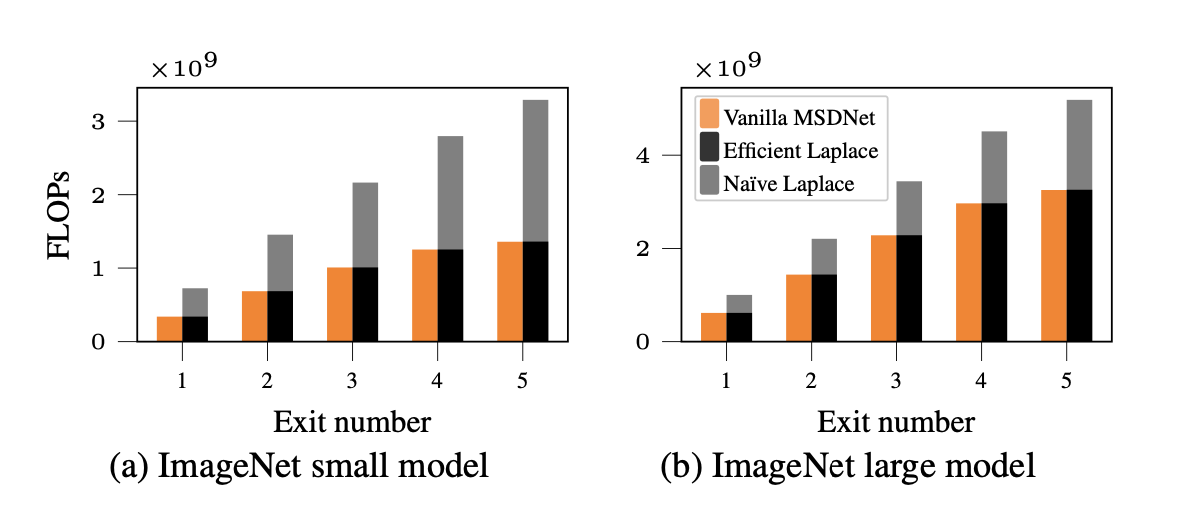
\includegraphics[width=0.5\linewidth]{Screenshot 2025-04-08 at 15.18.50.png}
        \label{fig:enter-label}
    \end{figure}
\end{frame}

\begin{frame}{Method}
    \scriptsize
    \begin{itemize}
        \item Last layer Laplace approximation for each intermediate classifier of the DNN

        \item Final prediction:
              \[
                  \hat{\mathbf{y}}_i = \frac{1}{n_{\text{MC}}} \sum_{l=1}^{n_{\text{MC}}} \text{softmax}(\hat{\mathbf{z}}_i^{(l)})
              \]

        \item Laplace implementation has cost:
              \[
                  {\text{FLOPs}_{\text{efficient}}} = 2c n_{\text{MC}} + 2p^2 + 5p + 2
              \]
              {\footnotesize \quad ($c$: number of classes, $p$: feature dimensionality, $n$: number of MC samples)}

        \item Gaussian distribution:
              \[
                  p(\hat{\mathbf{z}}_i \mid \mathbf{x}_i) = \mathcal{N}(\hat{\mathbf{W}}_{\text{MAP}}^\top \hat{\boldsymbol{\phi}}_i, \, (\hat{\boldsymbol{\phi}}_i^\top \mathbf{V} \hat{\boldsymbol{\phi}}_i) \mathbf{U})
              \]
              \[
                  \mathbf{V}^{-1} \otimes \mathbf{U}^{-1} = \mathbf{H}^{-1}
              \]

        \item Samples:
              \[
                  \hat{\mathbf{z}}_i^{(l)} = \hat{\mathbf{W}}_{\text{MAP}}^\top \hat{\boldsymbol{\phi}}_i + (\hat{\boldsymbol{\phi}}_i^\top \mathbf{V} \hat{\boldsymbol{\phi}}_i)^{\frac{1}{2}} (\mathbf{L} \mathbf{g}^{(l)})
              \]
              {\footnotesize \quad $\mathbf{g}^{(l)} \sim \mathcal{N}(0, \mathbf{I})$ and $\mathbf{L}$ is the Cholesky factor of $\mathbf{U}$}

        \item Temperature scaling is recommended for well-calibrated predictions
    \end{itemize}
\end{frame}

\begin{frame}{Uncertainty}
    \begin{itemize}
        \item The uncertainty should be high for the model to be able to recognize these samples as ‘tricky’, and continue their evaluation to the next block.
        \item For paper model these samples have a high uncertainty, while the vanilla MSDNet is overconfident.
    \end{itemize}
    \begin{figure}
        \centering
        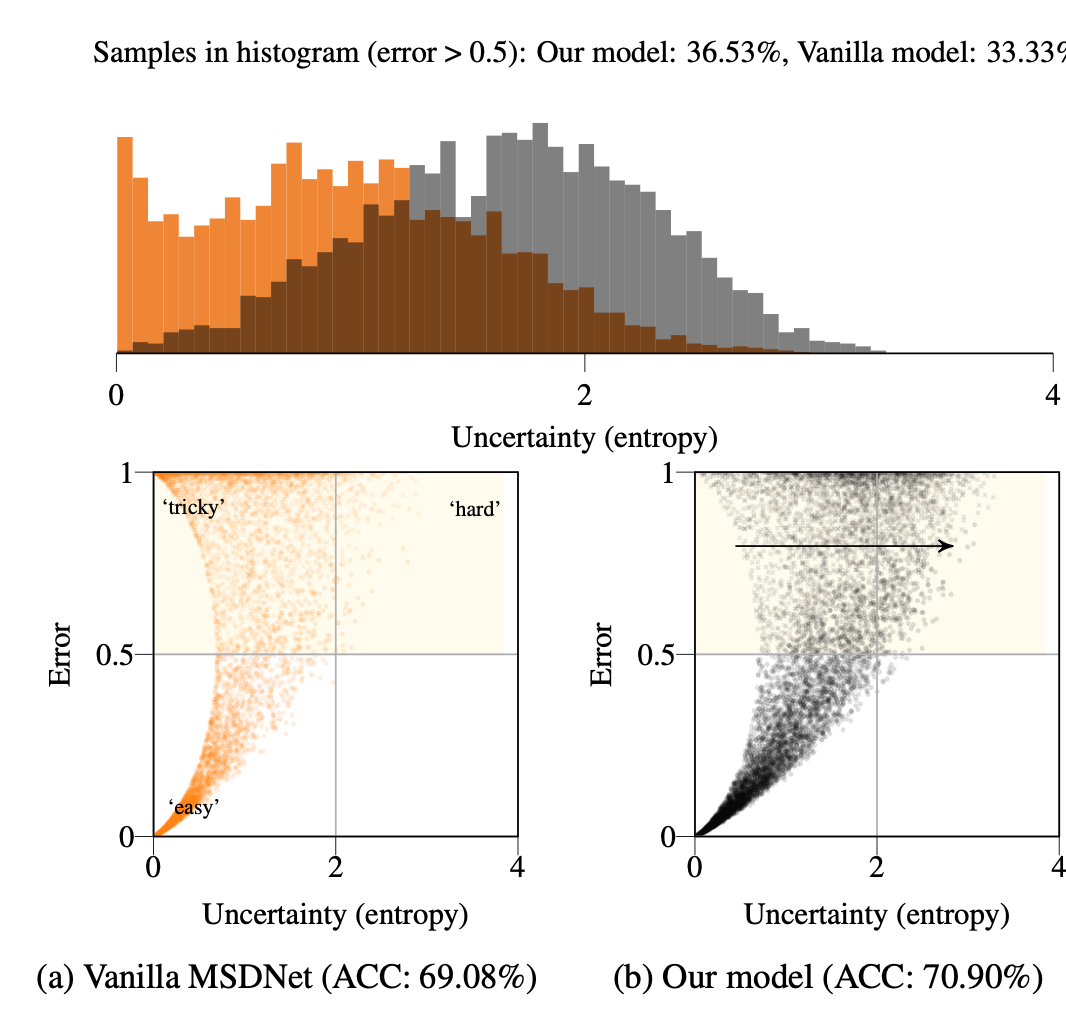
\includegraphics[width=0.35\linewidth]{Screenshot 2025-04-08 at 15.25.23.png}
        \label{fig:enter-label}
    \end{figure}
\end{frame}

\begin{frame}{Ensamble prediction}
    \[
        p_k^{\text{ens}}(\hat{\mathbf{y}}_i \mid \mathbf{x}_i) =
        \frac{1}{\sum_{l=1}^{k} w_l} \sum_{m=1}^{k} w_m \, p_m(\hat{\mathbf{y}}_i \mid \mathbf{x}_i)
    \]

    \vspace{1mm}
    Weights \( w \) are the computational costs in FLOPs up to classifier \( m \)

    \vspace{3mm}
    \begin{itemize}
        \item Early exiting decisions based on model predicted confidence (referred to as MIE)
        \item Thresholds for exiting are calculated on the validation set. Different for every layer (not included in paper)
    \end{itemize}

\end{frame}

\begin{frame}{Results}

    \begin{figure}
        \centering
        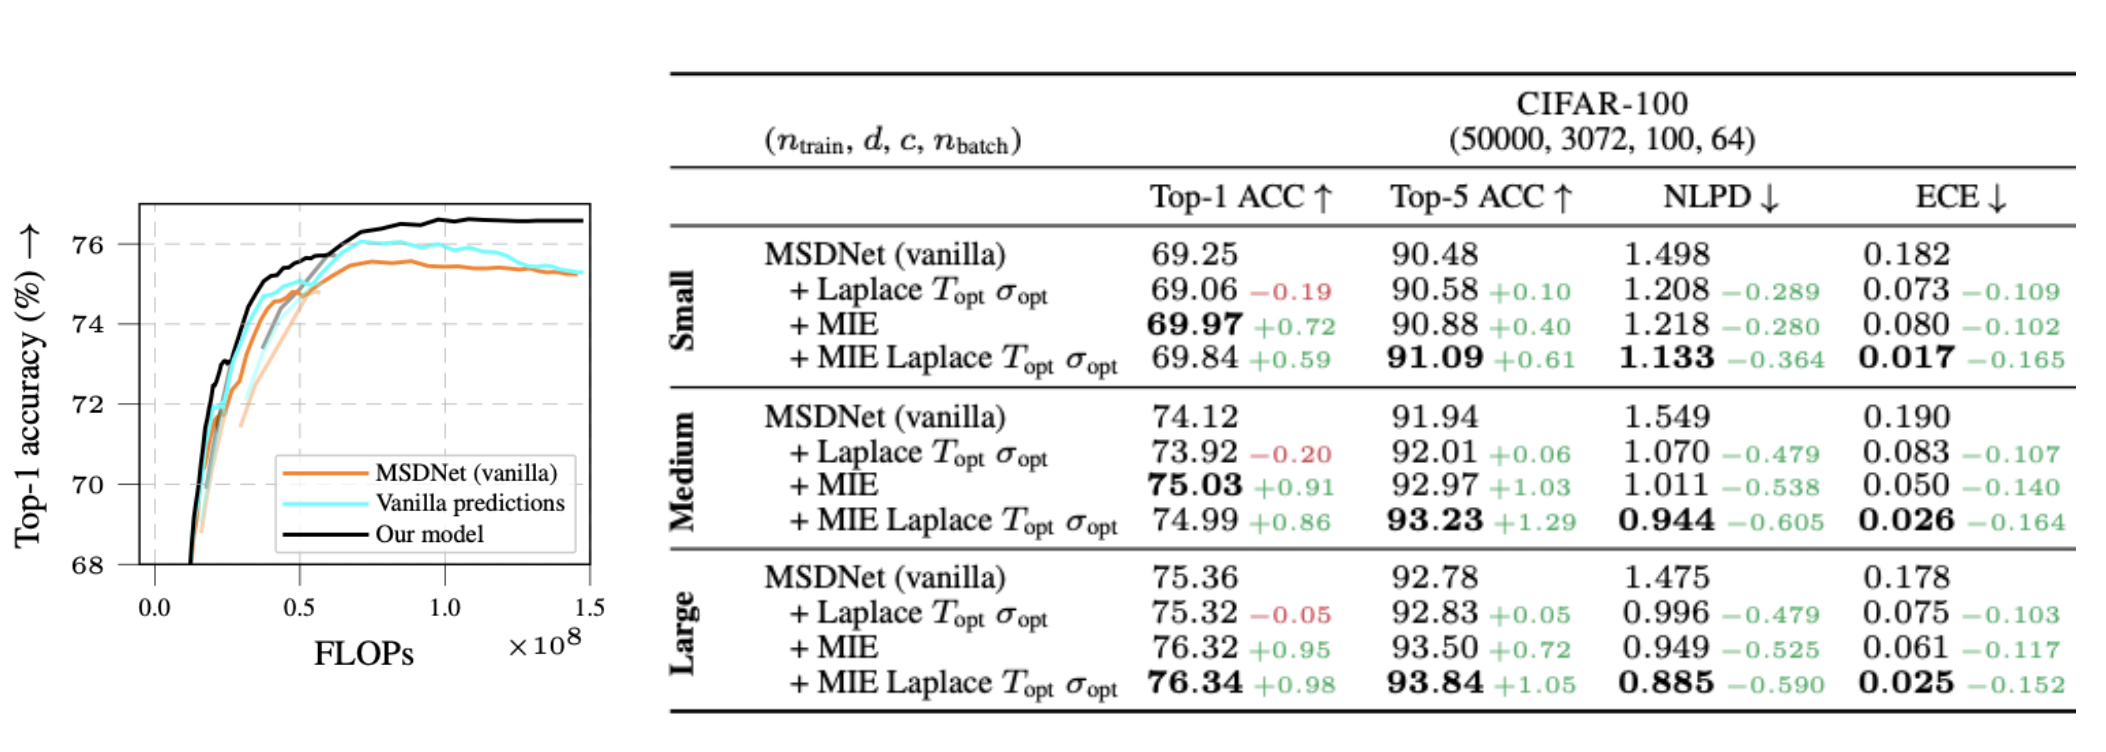
\includegraphics[width=0.8\linewidth]{Screenshot 2025-04-08 at 15.40.28.png}
        \caption{Enter Caption}
        \label{fig:enter-label}
    \end{figure}
    \begin{itemize}
        \item Improving confidence margins in teacher model makes for more efficient knowledge transfer in early exit training
        \item Implementing confidence margins in student model can increase accuracy

    \end{itemize}
\end{frame}

\begin{frame}{For our use}
    \begin{itemize}
        \item Improving confidence margins in teacher model makes for more efficient knowledge transfer in early exit training
        \item Implementing confidence margins in student model can increase accuracy

    \end{itemize}
\end{frame}